\chapter{General framework of \smtrat}
\label{chapter:generalframework}
\smtrat is a \Cpp library consisting of a collection of
SMT-compliant implementations of methods for solving non-linear real
arithmetic (NRA) formulas, we refer to as modules. These modules can be 
combined to (1) a theory solver in order to extend the supported logics of an
existing SMT solver by NRA or (2) an SMT solver for NRA. The latter is 
especially intended to be a testing environment for the development 
of SMT-compliant implementations of further methods tackling NRA. Here,
the developer must only implement the given interfaces of an \smtrat 
module and does not need to care about parsing input files, transforming
formulas to conjunctive normal form or embedding a SAT solver in order
to solve the Boolean skeleton of the given formula. Instead, \smtrat
provides this and more features, such as lemma exchange and bound
extraction, which we will explain in Section~\ref{}.

\smtrat defines three types of components (see Figure 
\ref{fig:framework}): the \emph{manager}, the \emph{strategy} and, as already mentioned, \emph{modules}. 
In addition, a frontend (1) provides the interfaces to an extern SMT 
solver or (2) parses the input file to a non-linear real arithmetic 
formula, we denote in the following just as formula.
In this section we first describe the functionality of a module and,
then, show how the manager composes different modules according to a
strategy to a solver.

\section{The \moduleClass class.} A module $m$ contains a set of
formulas, called its \emph{set of received formulas} denoted by 
$\Crcv(m)$. The main
procedure of a module  is \texttt{isConsistent()} and either decides
whether $\Crcv(m)$ is satisfiable or not returning \SAT or \UNSAT,
respectively, or returns \UNKNOWN. Note, that a set of formulas is
semantically defined by their conjunction. We can manipulate the set
of received formulas by adding (removing) formulas $\varphi$ to (from)
it with \texttt{add($\varphi$)} (\texttt{remove($\varphi$)}). Usually, 
$\Crcv(m)$ is only changed slightly between two consecutive 
\texttt{isConsistent()} calls, hence, the solver's performance can be significantly improved if the modules can
make use of the results of previous checks, that is they support
\emph{incrementality} and \emph{backtracking}. In case that the module
determines the unsatisfiability of $\Crcv(m)$, it is expected to compute
at least one preferably small \emph{infeasible subset} $\Cinf(m)\subseteq
\Crcv(m)$. Moreover, a module has the possibility to name lemmas, which
are formulas being tautologies, that is they hold for all assignments
of the variables occuring in them. These lemmas should encapsulate
information which can be extracted from a module's internal state and
propagated among other \smtrat modules. Furthermore, \smtrat provides
the feature that a module itself can ask other modules for the
satisfiability of a set of formulas, called its \emph{set
of passed formulas} denoted by $\Cpass(m)$, using the procedure \texttt{runBackends()} which
is controlled by the manager. 

\begin{figure}[t]
\caption{A snapshot of an \smtrat composition embedded in an SMT solver.}
\begin{center}
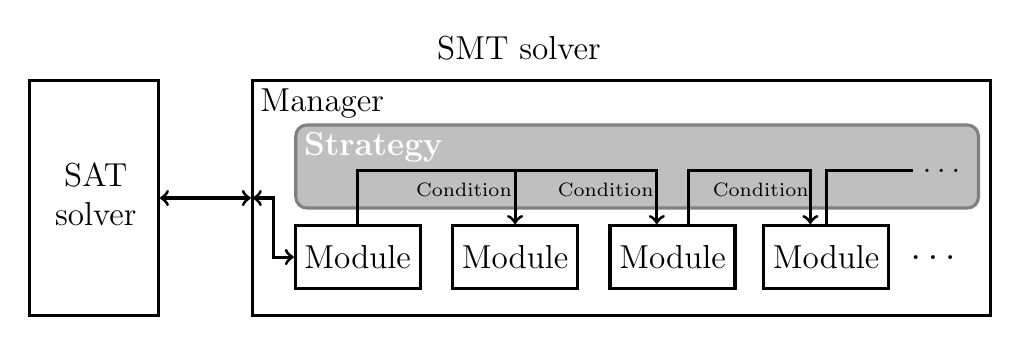
\begin{tikzpicture}[every node/.style={rectangle}, text centered, bend angle=15, scale=1, line width=.4mm]
	\node[] (smtsolver) at (-2.5, 2.2) {\large SMT solver};
	\node[draw, minimum height=85pt, text width=40pt] (satsolver) at (-7.9, 0.3) {\large\begin{tabular}{c}SAT \\ solver\end{tabular}};
	\node[draw, minimum height=85pt, text width=260pt] (manager) at (-1.2, 0.3) {};
	\node[] (managerText) at (-5, 1.5) {\large Manager};
	\node[fill=lightgray,draw=gray, rounded corners, minimum height=30pt, text width=240pt] (strategy) at (-1,.7) {};
	\node[] (strategyText) at (-4.35, .95) {\large\bf \color{white} Strategy};
	\draw[<->] (-5.36,-.45) -- (-5.62,-.45) -- (-5.62,.3) -- (-5.88,.3);
	\draw[->] (-4.55,-.03) -- (-4.55,.65) -- (-.75,.65) -- (-.75,-.03);
	\node[] (strategyText) at (-1.4, .4) {\scriptsize Condition};
	\draw[->] (-2.55,.65) -- (-2.55,-.03);
	\node[] (strategyText) at (-3.2, .4) {\scriptsize Condition};
	\draw[->] (-.35,-.03) -- (-0.35,.65) -- (1.2,.65) -- (1.2,-.03);
	\node[] (strategyText) at (.57, .4) {\scriptsize Condition};
	\draw (1.4,-.03) -- (1.4,.65) -- (2.5,.65);
	\node[] (dotsa) at (2.9,.65) {\large \ldots};
	\node[draw, minimum height=23pt] (moduleAText) at (-4.55, -.45) {\large Module};
	\node[draw, minimum height=23pt] (moduleBText) at (-2.55, -.45) {\large Module};
	\node[draw, minimum height=23pt] (moduleCText) at (-.55, -.45) {\large Module};
	\node[draw, minimum height=23pt] (moduleDText) at (1.4, -.45) {\large Module};
	\node[] (dotsc) at (2.8, -.45) {\Large \ldots};
	\path[<->] (satsolver.0) edge[] node[left] {} (manager.180);
\end{tikzpicture}

\end{center}
\label{fig:framework}
\end{figure}

\section{The \managerClass and the \strategyClass class} A
\emph{strategy} is a directed tree $T:=(V, E)$ with a set $V$ of
module (instances) as nodes and $E\subseteq V\times \Omega\times V$,
where $\Omega$ is a set of conditions. The \emph{manager} contains the
strategy and the input formula $C_{input}$, either received by a prefexed solver
or parsed from an example file. Furthermore, it maintains the
allocation of module as follows. Initially, the manager calls the method
\texttt{isConsistent()} of the module $m_r$ given by the root of
the strategy with $\Crcv(m_r) = C_{input}$ being the set of received formulas of this
module. Whenever a module $m\in V$ calls
\texttt{runBackends()}, with $\Cpass(m)$ being its set of passed
formulas, the manager calls \texttt{isConsistent()} of each module
$m'$ with \Crcv(m') = \Cpass(m) being its set of received formulas, for which
an edge $(m, \omega, m')\in E$ exists such that $\omega$ holds for
$\Cpass(m)$, and passes the results back to $m$. Furthermore, it also
passes back the infeasible subsets and lemmas provided by the invoked
modules. The module $m$ can now benefit in its solving and reasoning
process from this shared information.
%In the following we write short $(m, m')$ for $(m, \omega, m)$ if 
%$\omega = \True$.

%A complete SMT solver for NRA can be achieved as follows.
%The root module \CNFM transforms its set of received formulas $\Crcv^{cnf}$ to an equisatisfiable set of clauses $\Cpass^{cnf}$ and calls \texttt{runBackends($\Cpass^{cnf}$)}. The backend is a SAT-solver module \SATM, which runs DPLL-style SAT-solving on the Boolean abstraction of the set of received clauses $\Crcv^{sat}$. \SATM might call \texttt{runBackends($\Cpass^{sat}$)} for partial Boolean assignments on the corresponding set of formulas $\Cpass^{sat}$; we refer to such a backend call as \emph{theory call}. The Boolean abstraction of the obtained infeasible subsets and lemmas are stored as additional clauses. Infeasible subsets and lemmas, which contain only formulas from $\Cpass^{sat}$, prune the Boolean search space and hence the number of theory calls. Smaller infeasible subsets are usually more advantageous, because they make larger cuts in the search space. Other types of lemmas contain new formulas, so-called \emph{inventive lemmas} (\emph{non-inventive} otherwise) and might enlarge the Boolean search space, but they can reduce the complexity of later theory calls. This way we can compose SMT solvers for RCF, e.g., using the simple strategy defined by the nodes $I_{\CNFM}$, $I_{\SATM}$ and $I_{\CADM}$ 
%and the edges $(I_{\CNFM}, I_{\SATM})$ and $(I_{\SATM}, I_{\CADM})$.

